\chapter{序論}
\thispagestyle{empty}
\label{ch:Introduction}
\minitoc


\newpage


%%=========================================================================================
\section{背景}\label{sec:Background}

地震や噴火,豪雨などの自然災害はいつどこで発生するか分からず,誰もがその被害にさらされる可能性がある.
特に日本は,世界のなかでも,それらの自然災害が発生しやすい環境にある.
例えば地震については,日本は地震の震源が集中するプレートの境界上に位置しており,
2000年から2009年の間に世界で発生したマグニチュード6.0以上の地震のうち,約20\%が日本で発生した\cite{内閣府2010}.
また,日本は活火山の集中する環太平洋造山帯にも位置しているため,世界の活火山の内の約7\%にあたる
111の活火山が日本に分布している\cite{気象庁2019a}\cite{内閣府2010}.
さらに,春と夏の間に停滞する梅雨前線や夏から秋にかけて毎年平均約10個接近してくる台風によって豪雨が発生する場合があり,
1年間の降水量が世界平均の約2倍に達している\cite{気象庁2019b}\cite{国交省2004}.

これらの自然災害が土砂災害を誘発することも多い\cite{国交省2007}.
例えば,2018年に発生した北海道胆振東部地震では震源地となった北海道の胆振地方中東部を中心として広い範囲で
土砂災害が発生した\cite{国交省2019}.
また,2018年の6月28日から7月8日にかけて,停滞していた前線と台風第7号の影響で発生した平成30年7月豪雨では,
西日本を中心とした全国的に広い範囲で記録的な豪雨となり,
多くの土砂災害が発生した\cite{気象庁2018}.
これらの土砂災害の様子を,図\ref{fig:LandslideExample}に示す.
図\ref{fig:LandslideN}に,2008年から2018年の間に発生した土砂災害の件数と,
それに伴う被害者数,家屋被災戸数を示す\cite{国交省2019}.
この表からわかる通り,日本においては,毎年平均1000件ほどの土砂災害が発生しており,
特に2018年には集計開始以降最多の3459件の土砂災害が発生した.
また,土砂災害の発生に伴い,多くの人的被害や家屋の損壊が発生していることも分かる.

\begin{figure}[b]
	\begin{center}
		\begin{tabular}{c}

			\begin{minipage}[b]{0.5\linewidth}
			\centering
			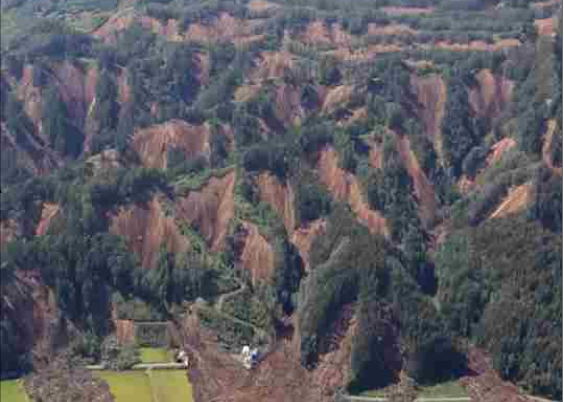
\includegraphics[width=5.5cm]{./Ch1_Introduction/Ch1_Fig/北海道胆振東部地震による土砂災害.PNG}
			\caption*{(a)地震による土砂災害}
			\end{minipage}

			\hfill

			\begin{minipage}[b]{0.5\linewidth}
			\centering
			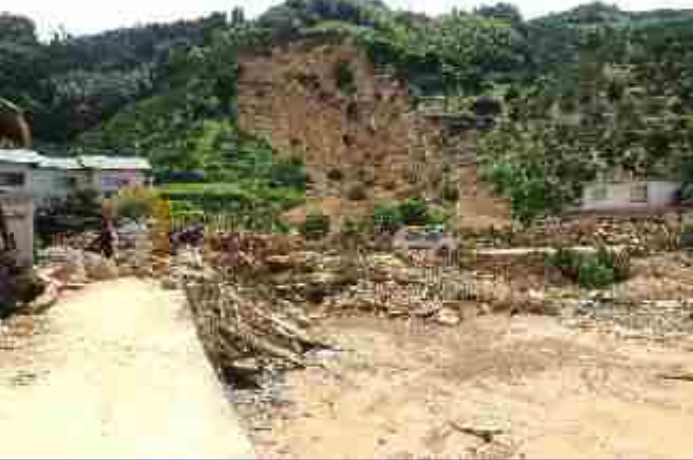
\includegraphics[width=5.5cm]{./Ch1_Introduction/Ch1_Fig/平成30年7月豪雨の土砂災害.png}
			\caption*{(b)豪雨による土砂災害}
			\end{minipage}

		\end{tabular}
	\caption{自然災害に誘発された土砂災害の例 \cite{国交省2019}}\label{fig:LandslideExample}	
	\end{center}
\end{figure}

% 土砂災害の写真をその災害を記述した箇所の真下に配置し,
% 2008年から2018年までの土砂災害による被害を示したグラフを隣のページに確実に配置する
\clearpage

\begin{figure}[p]
	\begin{center}

		\begin{minipage}[b]{0.9\linewidth}
		\centering
		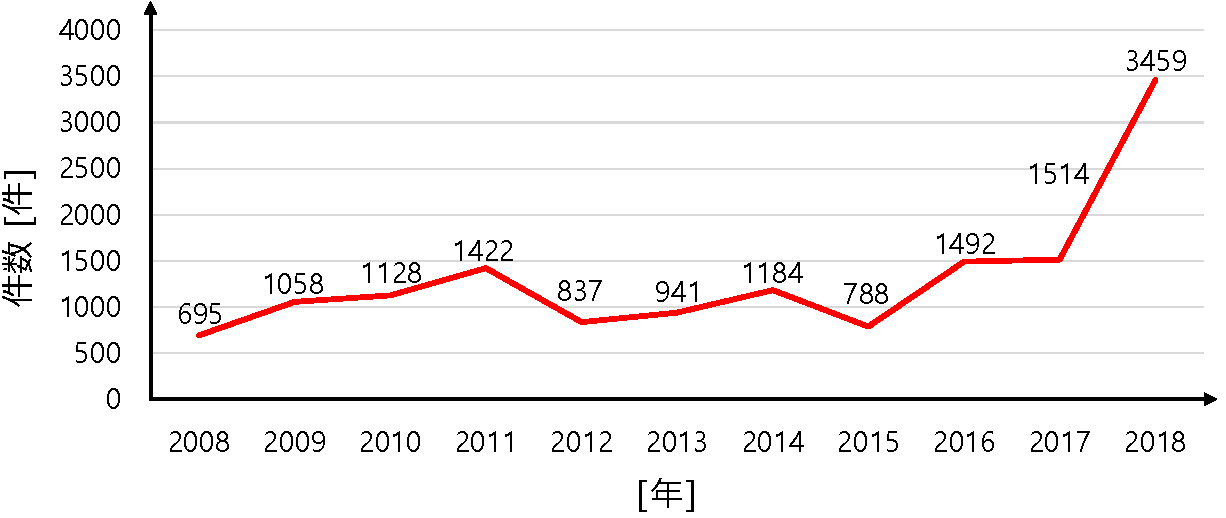
\includegraphics[width=12cm]{./Ch1_Introduction/Ch1_Fig/土砂災害発生件数.pdf}
		\vspace{-3mm}
		\caption*{(a)土砂災害発生件数}
		\end{minipage}\\

		\begin{minipage}[b]{0.9\linewidth}
		\centering
		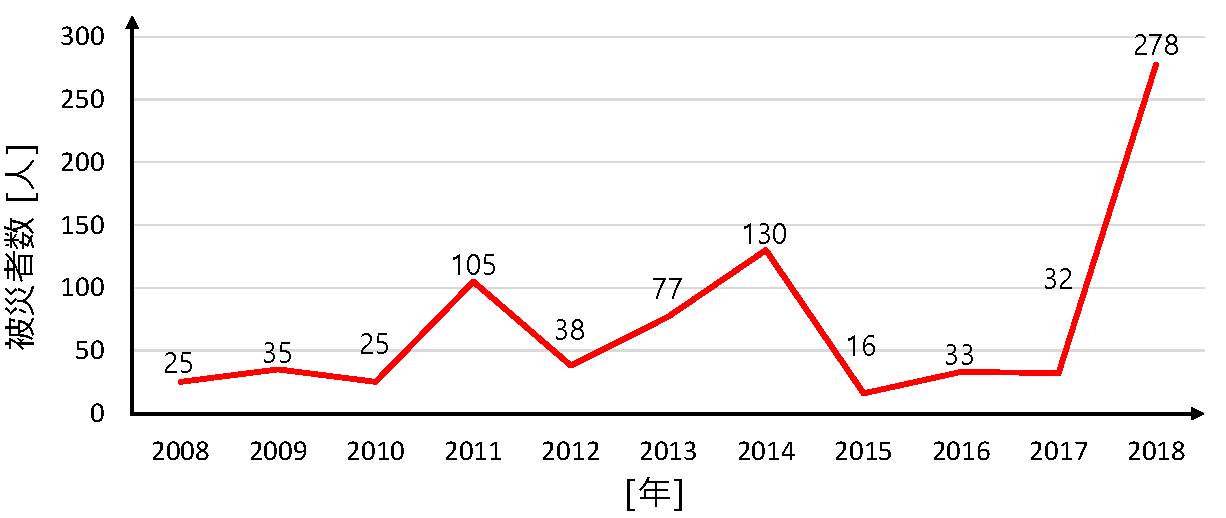
\includegraphics[width=12cm]{./Ch1_Introduction/Ch1_Fig/土砂災害の人的被害.pdf}
		\vspace{-3mm}
		\caption*{(b)土砂災害の人的被害(死者・行方不明者・負傷者数の合計)} 
		\end{minipage}\\

		\begin{minipage}[b]{0.9\linewidth}
		\centering
		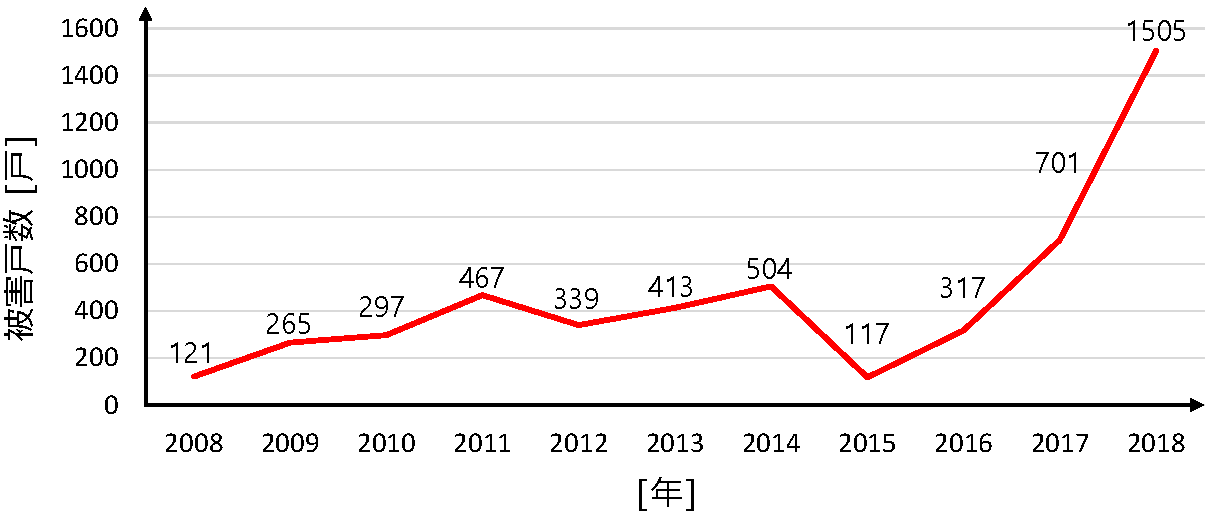
\includegraphics[width=12cm]{./Ch1_Introduction/Ch1_Fig/土砂災害の家屋被害戸数.pdf}
		\vspace{-3mm}
		\caption*{(c)土砂災害の家屋被害戸数} 
		\end{minipage}

	
	\caption{土砂災害の被害(\cite{国交省2019}を参考に作成)}\label{fig:LandslideN}
	\end{center}
\end{figure}

\clearpage

土砂災害が発生した場合に発生する被害を最小限にするためには,
人命救助やライフラインの復旧などを早急に行う必要がある\cite{国交省2016}.
例えば,崩壊してきた土砂や倒壊した家屋の下敷きになった人を救助する必要があるが,
被災者は3日間以上経過すると生存率が大幅に低下してしまう\cite{国交省2002}.
また,電力,水道,通信,道路等のライフラインが土砂災害によってその機能を停止した場合,経済的な損失を誘発してしまう\cite{豊田2008}\cite{豊田2010}.
人命救助や交通網の確保を早急に行うためには,迅速な復旧工事が必要となる.
そのためには,復旧工事において建設機械の使用が必要となるが,
土砂災害の発生した現場の地盤が軟弱な場合,
地盤が建設機械の重量に耐えられずに,建設機械が転倒してしまう可能性がある\cite{玉手2014}\cite{玉手2008}.
従って,まず最初に災害現場において建設機械の走破性を調査することが重要となる.


% \begin{figure}[b]
% 	\begin{center}
% 	\centering
% 	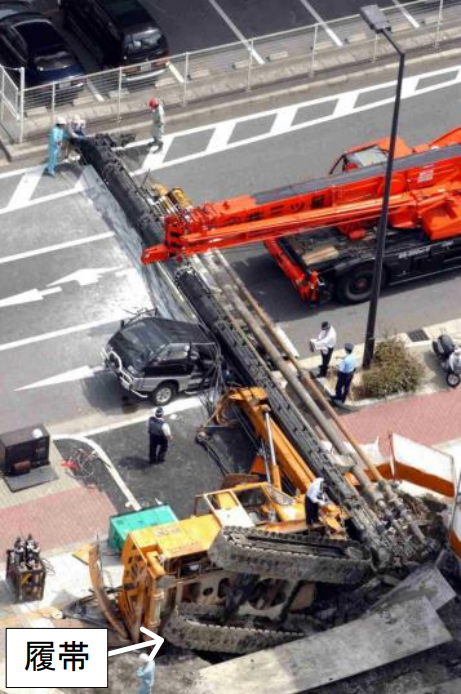
\includegraphics[width=7cm]{./Ch1_Introduction/Ch1_Fig/軟弱地盤のために転倒した建設機械c.PNG}
% 	\caption{軟弱地盤のために転倒した建設機械 \cite{玉手2008}}\label{fig:FalledConstructionMachinery}
% 	\end{center}
% \end{figure}

\clearpage


%%=========================================================================================
\section{先行研究}\label{sec:PreviousStudy}

\subsection{従来の走破性調査}\label{ssec:TraditionalMethod}

建設機械の走破性を調査する従来手法には,走破性を示す指標の1つであるコーン指数を計測する手法がある\cite{Perumpral1987}\cite{Mulqueen1977}.
コーン指数とは,コーンペネトロメータと呼ばれる器具を現場の地面に挿入し,その際に発生する土の抵抗力を,
コーンペネトロメータの上部についているメーターで読み取ることで得られる値である.
土の抵抗力が強いほど建設機械の走破性が高いので,
コーン指数が高いほど建設機械の走破性が高いと判定することができる.
コーンペネトロメータとそれを用いたコーン指数の測定の様子を図\ref{fig:ConeIndexMeasurement}に示す.
これまでコーン指数の測定は人の手で行われてきたが,災害現場では2次災害の危険が存在するため,
現場で人がコーンペネトロメータを挿入してコーン指数を測定することは大変危険である.
従って,無人でコーン指数を測定する手法が求められている.

\begin{figure}[b]
	\begin{center}
		\begin{tabular}{c} % 隣り合う図がずれないようにする

			\begin{minipage}[b]{0.45\linewidth}
			\centering
			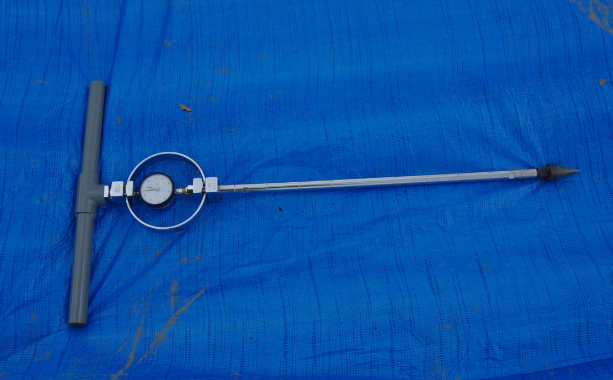
\includegraphics[width=8cm, angle=-90]{./Ch1_Introduction/Ch1_Fig/コーンペネトロメータa.PNG}
			\caption*{コーンペネトロメータ}
			\end{minipage}

			\hfill

			\begin{minipage}[b]{0.45\linewidth}
			\centering
			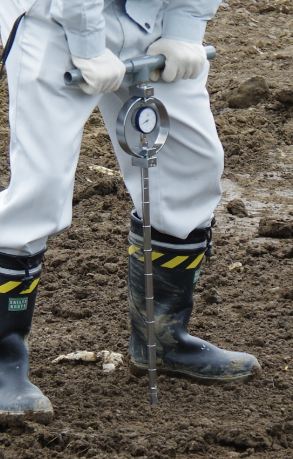
\includegraphics[height=8cm]{./Ch1_Introduction/Ch1_Fig/コーンペネトロメータb.PNG}
			\caption*{コーン指数の測定の様子}
			\end{minipage}

		\end{tabular}
	\caption{コーンペネトロメータを用いたコーン指数の測定}\label{fig:ConeIndexMeasurement}
	\end{center}
\end{figure}

\clearpage

\subsection{無人でのコーン指数の測定}\label{ssec:UnmannedMethod}

無人でコーン指数を測定する先行研究には,ロボットにコーン指数を測定する器具を搭載し,
遠隔操作にてこのロボットを,対象とする環境まで移動させ,この器具でコーン指数を測定する
手法が提案されている\cite{RobotWatch2002}\cite{古谷2016}\cite{Chhaniyara2012}\cite{Zacny2010}.
図\ref{fig:coneindex_measurement_by_robot}に,先行研究の1つの例を示す.
この例では,コーン指数を測定する器具として,簡易動的コーン貫入試験という器具をロボットに搭載して使用している.
この手法は,人の手によるコーン指数の測定を,遠隔操作できるロボットに
置き換えることによって無人でのコーン指数の測定を達成したが,測定器具を測定地点に1カ所ずつ接触させる必要があるため,
地盤が軟弱な場合や急勾配の斜面がある場合などの,ロボットが対象とする環境に移動することができない場合には,
コーン指数の測定を行うことができないという問題がある.
従って,ロボットが対象とする環境に移動することができない場合でも
コーン指数の測定を行うため,
非接触でコーン指数を推定する手法が必要となる.

\vspace{3cm}% 下にある図をページ下部にある空白部分のできるだけ中心に配置する

\begin{figure}[bh]
	\begin{center}
		\begin{tabular}{c}

			\begin{minipage}[b]{0.6\linewidth}
			\centering
			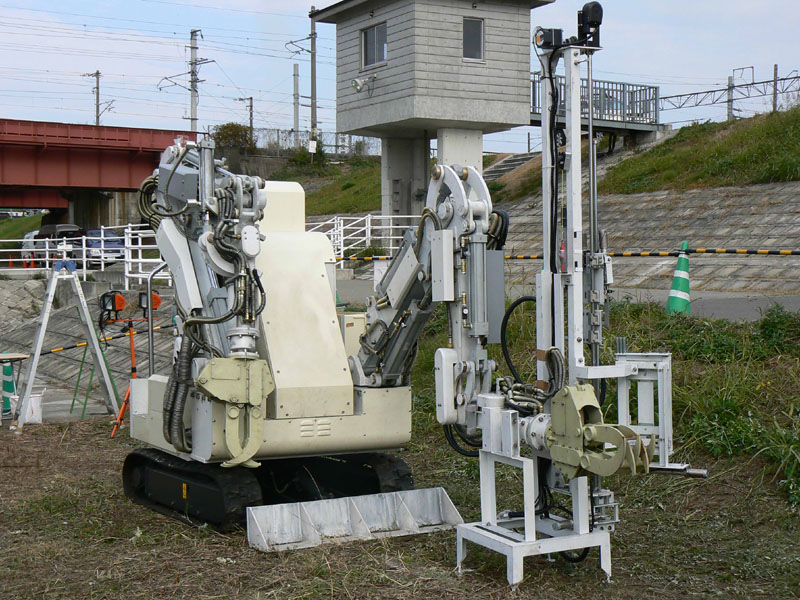
\includegraphics[height=5.5cm]{./Ch1_Introduction/Ch1_Fig/遠隔操作ロボット.jpg}
			\caption*{遠隔操作ロボット}
			\end{minipage}

			\hfill

			\begin{minipage}[b]{0.3\linewidth}
			\centering
			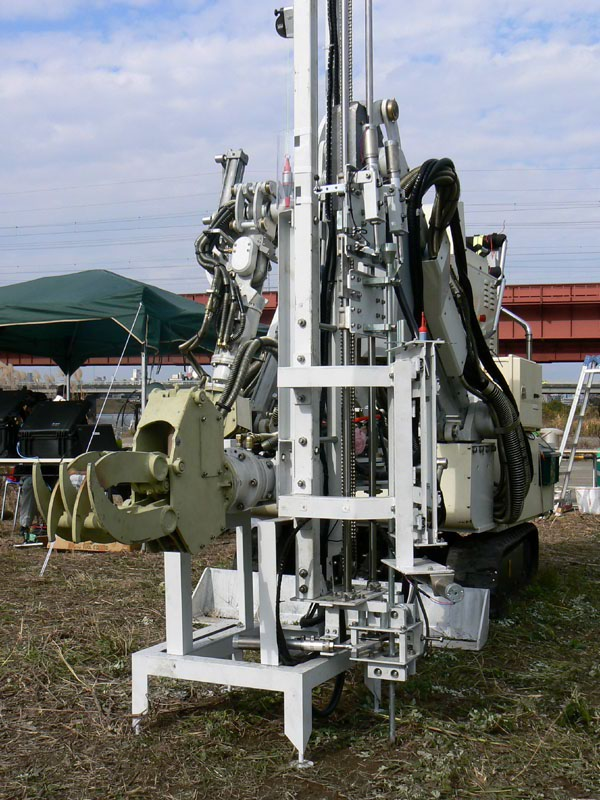
\includegraphics[height=5.5cm]{./Ch1_Introduction/Ch1_Fig/遠隔操作ロボットの簡易動的コーン貫入試験機.jpg}
			\caption*{簡易動的コーン貫入試験機}
			\end{minipage}

		\end{tabular}
	\caption{遠隔操作ロボットに搭載した簡易動的コーン貫入試験機を用いた無人でのコーン指数の測定 \cite{RobotWatch2002}}\label{fig:coneindex_measurement_by_robot}
	\end{center}
\end{figure}

\clearpage

\subsection{非接触計測によるコーン指数の推定}\label{ssec:NonContactMethod}

% 非接触でコーン指数を推定するために,画像を用いる手法が存在する.
% しかし,画像を用いて推定する手法では,土の表面の情報しか取得することができず,
% 深い部分にある土の強度の情報を取得することができない.
% ただし,一般的に,土は深いところにあるほど上の土の質量が増加するため締め固められることが多く,
% その場合,一番上にある一番軟らかい土のコーン指数が建設機械の重量に耐えられるならば,
% 深い部分にある土のコーン指数も当然建設機械の重量に耐える.
% 従って,土の表面にある一番軟らかい土のコーン指数だけを推定しても,
% 結果的には問題ないことになる.
% 本研究では,上記のような,深いところにある土ほど上の土に締め固められて固くなる土を想定することとする.
% 図\ref{fig:SoilFirmnessFeature}(a)に,本研究で想定する土の深さと固さの関係を,そして
% 図\ref{fig:SoilFirmnessFeature}(b)に,本研究で想定する土の深さとコーン指数の関係を示す.

% \vspace{3cm}% 下にある図をページ下部にある空白部分のできるだけ中心に配置する

% \begin{figure}[h]
% 	\begin{center}
% 		\begin{tabular}{c}

% 			\begin{minipage}[b]{0.5\linewidth}
% 			\centering
% 			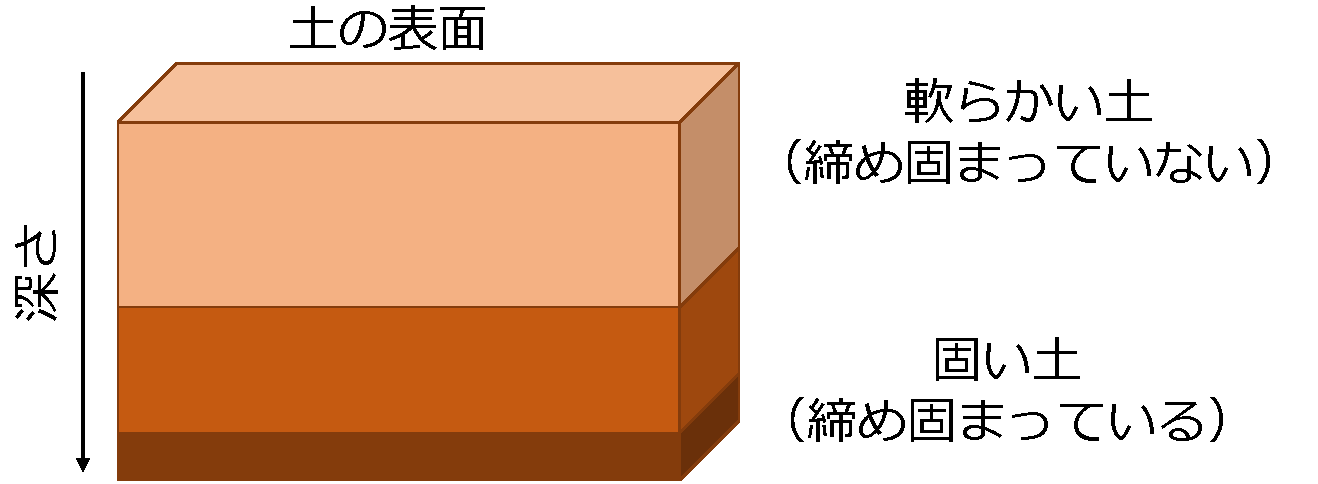
\includegraphics[height=3cm]{./Ch1_Introduction/Ch1_Fig/relationship_between_compaction_and_depth.pdf}
% 			\caption*{(a)土の深さと固さの関係}
% 			\end{minipage}

% 			\hfill

% 			\begin{minipage}[b]{0.5\linewidth}
% 			\centering
% 			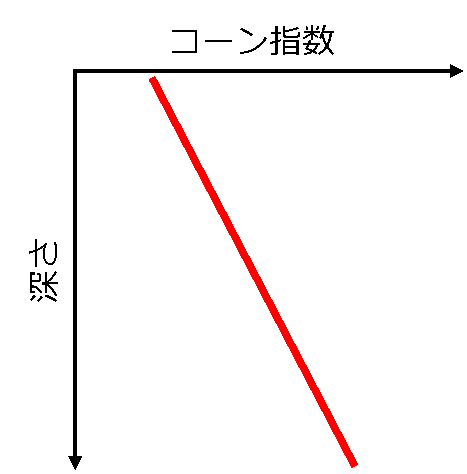
\includegraphics[height=3cm]{./Ch1_Introduction/Ch1_Fig/relationship_between_coneindex_and_depth.pdf}
% 			\caption*{(b)土の深さとコーン指数の関係}
% 			\end{minipage}

% 		\end{tabular}
% 	\caption{一般的な土の固さの特徴}\label{fig:SoilFirmnessFeature}
% 	\end{center}
% \end{figure}

% \clearpage

非接触計測によってコーン指数を推定する先行研究には,水が光を吸収する近赤外の波長帯を撮影した画像を用いてコーン指数を推定する手法が提案されている\cite{Fernandez2015}\cite{Rankin2010}.
図\ref{fig:images_for_coneindex_estimation}(a)に,この先行研究で使用された近赤外線画像を示す.
この手法では画像を用いることによって,非接触計測によるコーン指数を推定することができるが,土に含まれる水の量を示す指標である含水比にのみ注目し,
含水比以外でコーン指数に影響を与える土の種類には注目していないため,推定されたコーン指数の精度が低いという問題がある.

一方,スペクトル画像から得られた分光反射率スペクトルを用いてコーン指数を推定する手法も提案されている\cite{Sopher2016}.
図\ref{fig:images_for_coneindex_estimation}(b)に,この先行研究で使用された分光反射率スペクトルを示す.
しかし,この手法は水が光を吸収する波長帯を除いた分光反射率スペクトルを用いているため,結果的に土の種類にのみ注目して
逆に含水比を無視している.
従って,この手法でも推定されたコーン指数の精度が低いという問題がある.
従って,土の種類と含水比の双方に注目した,非接触計測によるコーン指数の推定手法が必要である.

\begin{figure}[p]
	\begin{center}
		\begin{tabular}{c}

			\begin{minipage}[b]{0.9\linewidth}
			\centering
			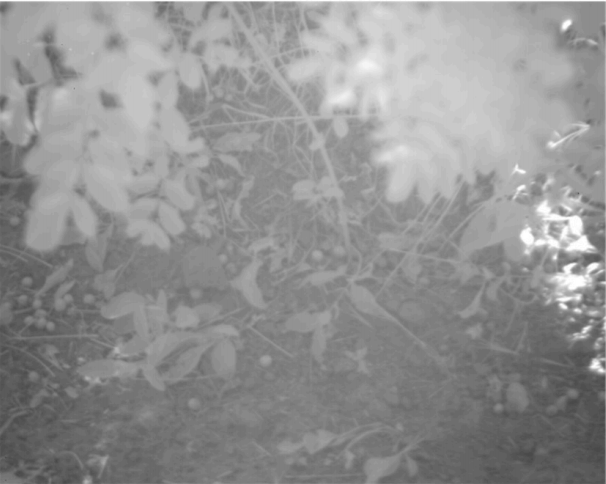
\includegraphics[width=6cm]{./Ch1_Introduction/Ch1_Fig/先行研究_コーン指数推定のための近赤外線画像.PNG}
			\caption*{(a)コーン指数推定のための近赤外線画像 \cite{Fernandez2015}}
			\vspace{1cm} % 上下の図が近づきすぎないようにする
			\end{minipage}\\

			\begin{minipage}[b]{0.9\linewidth}
			\centering
			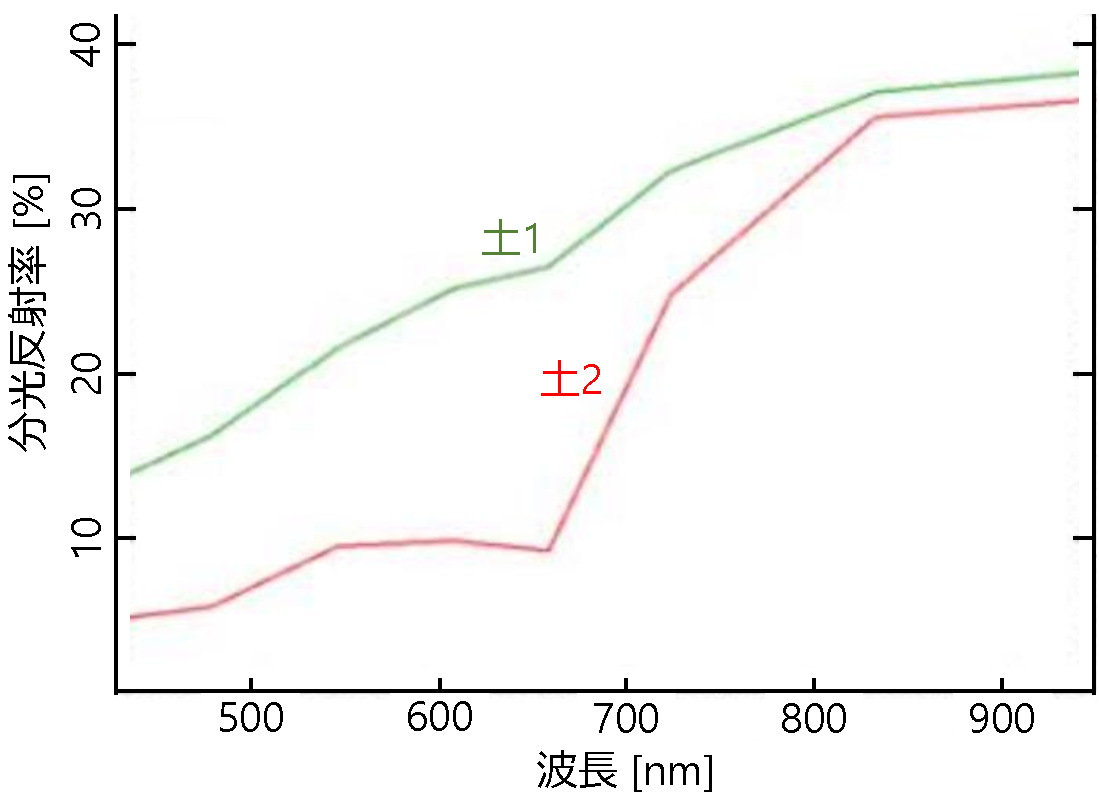
\includegraphics[width=6.6cm]{./Ch1_Introduction/Ch1_Fig/spectrum_difference_of_different_soiltypes.pdf}
			\caption*{(b)コーン指数推定のための分光反射率スペクトル \cite{Sopher2016}}
			\end{minipage}

		\end{tabular}
	\caption{非接触計測によるコーン指数の推定}\label{fig:images_for_coneindex_estimation}
	\end{center}
\end{figure}

\clearpage


%%=========================================================================================
%%=========================================================================================
\section{本論文の目的}\label{sec:Objective}

\ref{sec:Background}節において,土砂災害が発生した災害現場では,実際に建設機械を使用する前に走破性を調査する必要があることを述べた.
\ref{sec:PreviousStudy}節においては,災害現場での走破性の調査には,非接触にコーン指数を推定する手法が適していることを述べた.
また,コーン指数には土の種類と含水比の双方が大きく影響しているため,双方に注目する必要があるにも関わらず,
これまでの非接触なコーン指数の推定手法には双方に注目した手法がまだ存在しないことにも言及した.
従って,本研究の目的を,以下の通りとする.

\vspace{5pt}
\begin{itembox}[c]{目的}
\begin{center}
土の種類と含水比の双方に注目した\\画像による建設機械のためのコーン指数の推定
\end{center}
\end{itembox}
\vspace{5pt}

本研究では,まず画像を用いて土の種類の識別と含水比の推定を行い,
それらからコーン指数を推定することを目指す.
土の種類の識別と含水比の推定を行うため,本研究ではスペクトル画像を使用する.
スペクトル画像とは,撮影する対象物からの反射光を分光させて,分光された波長ごとの強度を2次元平面で表示した画像である\cite{Tominaga1999}.
スペクトル画像のイメージを図\ref{fig:spectral_image}に示す.
この図において,x軸,y軸方向は各波長ごとの2次元平面の座標を表しており,
z軸は波長方向を表している.
そして,z軸方向に積み重なった2次元平面の枚数が,分光された波長の数を表している.
そこで,スペクトル画像のそれぞれの波長の強度を示す2次元平面から算出される分光反射率を並べると,
分光反射率スペクトルを取得することができる.
本研究では,この分光反射率スペクトルから土の種類の識別と含水比の推定を実施する.

\begin{figure}[bh]
	\begin{center}
	\centering
	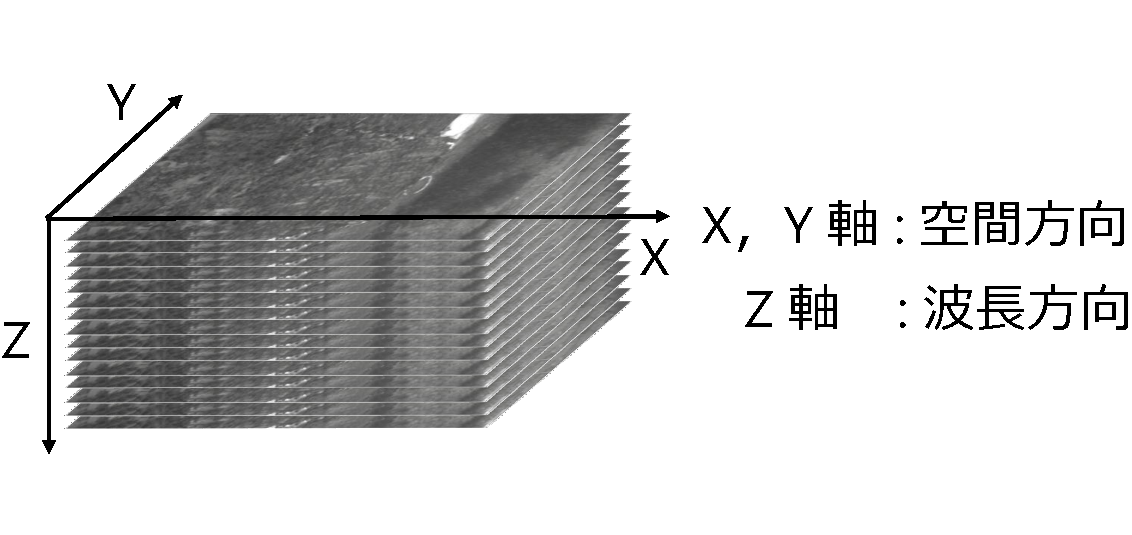
\includegraphics[width=8cm]{./Ch1_Introduction/Ch1_Fig/SpectralImage.pdf}
	\caption{スペクトル画像}\label{fig:spectral_image}
	\end{center}
\end{figure}

\clearpage


%%=========================================================================================
\section{本論文の構成}\label{sec:Structure}

本論文は,全6章から構成されている.
本論文の構成を\mbox{図\ref{fig:MThesisConstitution}}に示す.

第\ref{ch:Introduction}章では,土砂災害の発生現場における走破性の調査の重要性と,
そのための非接触なコーン指数の推定手法の必要性について言及した.
そして,本研究においては,スペクトル画像から取得できる分光反射率スペクトルを用いて
土の種類の識別と含水比の推定を実施し,それらからのコーン指数の推定を目標とすることを述べた.

第\ref{ch:SoilTypeDiscrimination}章では,スペクトル画像を用いて土の種類を識別する手法について述べる.
本研究では,土の種類ごとに分光反射率スペクトルが異なっていることを利用し,
スペクトル画像から取得した分光反射率スペクトルを分類することで土の種類を識別する.

第\ref{ch:WaterContentEstimation}章では,スペクトル画像を用いて含水比を推定する手法について述べる.
本研究では,水が近赤外の幅広い波長帯の光を吸収することを利用する.
スペクトル画像から水が光を吸収する近赤外の波長帯と光を吸収しない波長帯の分光反射率を取得し,
その2つの波長帯の分光反射率を比較することで含水比を推定する.

第\ref{ch:ConeIndexEstimation}章では,識別した土の種類と推定した含水比からコーン指数を推定する手法について述べる.
本研究では,土の種類ごとに含水比とコーン指数が一意の関係にあることを利用し,
第\ref{ch:SoilTypeDiscrimination}章で識別した土の種類と
第\ref{ch:WaterContentEstimation}章で推定した含水比から
コーン指数を推定する.

第\ref{ch:VerificationExperiment}章では,屋外のスペクトル画像から走破性を判定することによって,
提案手法の有効性を確認するために実施した検証実験について述べる.
具体的には,屋外のスペクトル画像から本研究の提案手法を用いて識別した土の種類,
推定した含水比,およびコーン指数と,実際の土の種類,含水比,およびコーン指数を比較することによって,
提案手法の有効性を確認する.

第\ref{ch:Conclusion}章では,本論文のまとめと今後の展望を述べる.

\begin{figure}[pb]
	\begin{center}
	\centering
	\includegraphics[width=10cm]{./Ch1_Introduction/Ch1_Fig/ThesisConstitution.pdf}
	\caption{修論構成}\label{fig:MThesisConstitution}
	\end{center}
\end{figure}

\clearpage


%%%%%%%%%%%%%%%%%%%%%%%%%%%%%%%%%%%%%%%%%%%%%%%%%%%%%%%%%%%%%%%%%%%%%%%%%%%%%%%
%%% Local Variables:
%%% mode: katex
%%% TeX-master: "../thesis"
%%% End: